\documentclass[a4paper,fleqn,12pt]{article}

\usepackage[utf8]{inputenc}
\usepackage[bulgarian]{babel}
\usepackage{amsmath}
\usepackage{amssymb}
\usepackage{booktabs}
\usepackage{fancyhdr}
\usepackage{amsthm}
\usepackage{graphicx}
\usepackage{color}

%\pagestyle{fancy}
%\fancyhf{}
%\lhead{\rightmark}
%\rhead{\thepage}
%\cfoot{}
%\renewcommand{\headrulewidth}{0pt}

%\sloppy
%\definecolor{lightgray}{gray}{0.5}
%\setlength{\parindent}{0pt}


\begin{document}
\begin{titlepage}
	\setlength{\parindent}{0pt}
	\large
\centering
Технически университет -  София \par
Факултет по приложна математика и информатика \par
\vspace{2cm}

{\huge Курсова работа \par}

\vspace{2cm}

\vspace{1cm}
{\LARGE\scshape Числено моделиране с обикновенни диференциални уравнения \par}



\vfill

\begin{minipage}[t]{.5\linewidth}
	Студент: \\
	Кристиян Кръчмаров
\end{minipage}%
\begin{minipage}[t]{.5\linewidth}
	\raggedleft
	Преподавател:\\
	доц. д-р. Богдан Гилев
\end{minipage}

\vspace{2cm}
\raggedright

\end{titlepage}
\tableofcontents
\newpage

\section{Задачи}
\subsection{Задача 1}
Да се реши системата по Рунге - Кута: 
	\begin{gather}
		\begin{array}{|l@{}}
		\frac{dy_1}{dx} = y_2 \\
		\frac{dy_2}{dx} = f(x,y_1,y_2)
		\end{array} \qquad \qquad  \text{при} \qquad \qquad 
		\begin{array}{|l@{}}
		y_1(0) = 0\\
		y_2(0) = y_{20}
		\end{array}\\
		\text{където:} \nonumber \\
		f(x,y_1,y_2) = -axy_2 - x^2y_1 \quad a=0.05 \quad y_{20} = \frac{1}{6} \nonumber
	\end{gather}

\subsection{Задача 2}
Да се сведе до система и да се реши по метода на матричната експонента уравнението при нулеви начални условия
	\begin{equation}
	y''+3y'=xe^{-2x}
	\end{equation}

\subsection{Задача 3}
Да се реши граничната задача по метода на крайните разлики
	\begin{equation}
	x'' + \frac{1}{t} x' + \left( \frac{16}{t^2}\right) x = \sin \left( \frac{1}{t^2}\right) \quad t \in [1;4]; \, x(1) = -0.3 ; \, x(4) = 0.4
	\end{equation}

\subsection{Задача 4}
Да се реши граничната задача по метода на стрелбата
	\begin{equation}
	x'' + \frac{1}{t} x' + \left( \frac{16}{t^2}\right) x = \sin \left( \frac{1}{t^2}\right) \quad t \in [1;4]; \, x(1) = -0.3 ; \, x(4) = 0.4
	\end{equation}

\newpage
\section{Решения}
\subsection{Задача 1}
Mетодът на Рунге-Кута от 4ти ред се използва за числено решение на система 
обикновенни диференциални уравнения от вида.
	\begin{gather*}
		\begin{array}{|l@{}}
		\frac{dy_1}{dx} = g(x,y_1,y_2) \\
		\frac{dy_2}{dx} = f(x,y_1,y_2)
		\end{array}
		\qquad \qquad  \text{при} \qquad \qquad 
		\begin{array}{|l@{}}
		y_1(x_0) = y_{10}\\
		y_2(x_0) = y_{20}
		\end{array} \\
		\text{където:}  \\
		y_1 = y_1(x) ; \, y_2 =y_2(x) 
	\end{gather*}
Методът се базира на апроксимация на следващата стойност на фунцкията, 
като използва няколко променливи за изчисляване на инкрементацията. 
При Метод на Рунге-Кута от 4ти ред се използват следните променливи
	\begin{gather*}
		Y_i = \{y_1,y_2 \} \\
		k_1 = h \cdot f(x_i,Y_i)\\
		k_2 = h \cdot f \left(x_i + \frac{h}{2},  Y_i + \frac{h}{2}\cdot k_1\right)\\
		k_3 = h \cdot f \left(x_i + \frac{h}{2},  Y_i + \frac{h}{2}\cdot k_2 \right)\\
		k_4 = h \cdot f \left(x_i + h,  Y_i + h \cdot k_3\right)\\
		Y_{i+1} = Y_{i} + \frac{h}{6} \left( k_1 +2k_2 + 2k_3 + k_4\right)\\
\end{gather*}
където $Y_{i}$ e предходното приближение, а $Y_{i+1}$ e текущoтo приближениe. \\
	\newpage
\begin{verbatim}
function firstTask
h=0.1;%стъпка
x=0:h:10;
n=length(x);%итерации
y(1,1)=0; y(2,1) = 0.16;%начални условия
for i=1:(n-1)
    k1=h*system (x(i), y(1:2,i));
    k2=h*system (x(i) + h/2, y(1:2, i) + h*k1/2);
    k3=h*system (x (i) + h/2, y(1:2, i) + h*k2/2);
    k4=h*system (x(i) + h, y(1:2, i) +h*k3);
    y(1:2, i+1)=y(1:2, i) + (h*(k1+2*k2+2*k3+k4))/6;
end
figure (1), plot (x,y (1, :),x,y(2,:));
legend('y_1', 'y_2','Location', 'best');
title('Решение на системата по Рунге-Кута');
end

function f = system (x, y)
    f(1,1)=y(2);
    f(2,1)=0.05*x*y(2)-x^2*y(1);
end
\end{verbatim}
\begin{center}
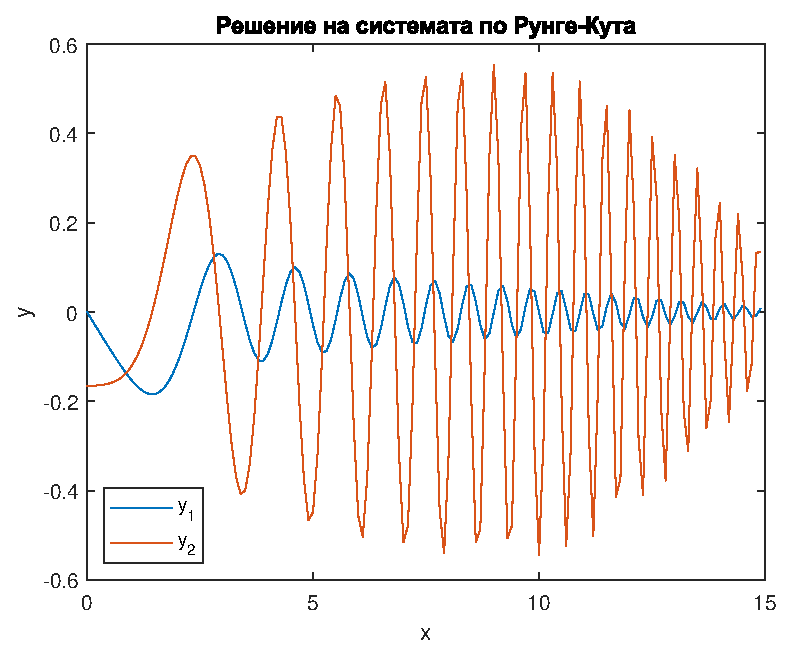
\includegraphics [width=4in]{firstTask_01.eps}
\end{center}

\newpage
\subsection{Задача 2}
Методът на матричната експонента се използва за числено решение на система обикновенни диференциални уравнения от вида 
	\begin{gather*}
		\frac{dy}{dx} = Ay + Bx
		\qquad \qquad  \text{при} \qquad \qquad 
      		y(x_0)=y_0 \\
	\end{gather*}
Матричната експонента се дефинира като безкраен матричен ред
\begin{equation*}
	e^{Ax} = E + \sum_{n=1} ^{\infty} \frac{A^n}{n!}
\end{equation*}
където $E$ е единичната матрица, а $A^n$ е произведението на А, n пъти.\\
В задачата уравнението се свежда до система с въвеждането на 
	\begin{gather*}
		\begin{array}{|l@{}}
			y_1=y\\
			y_2=y'
		\end{array} \implies 
		\begin{pmatrix} y_1 \\ y_2 \end{pmatrix}' = 
		\begin{pmatrix} 0 & 1 \\ 0 & -3 \end{pmatrix} 
		\begin{pmatrix} y_1 \\ y_2 \end{pmatrix} + 
		\begin{pmatrix} 0 \\ xe^{-2x} \end{pmatrix} \iff Y'=AY+B(x)\\ 
		Y'=\begin{pmatrix} y1 \\ y2 \end{pmatrix}' \qquad 
		A=\begin{pmatrix} 0 & 1 \\ 0 & -3 \end{pmatrix} \qquad 
		B(x)=\begin{pmatrix} 0 \\ xe^{-2x} \end{pmatrix} \qquad
		Y=\begin{pmatrix} y1 \\ y2 \end{pmatrix}
	\end{gather*}
Решението на уравнението се дава във вида
\begin{equation*}
	y(x)=e^{A(x-x_0)} y(x_0) + e^{Ax} \int_{x_0} ^{x} e^{-As} B(s) \ ds
\end{equation*}
което може да се дискретизира след полагане на $x_0 = kh, \, x = (k+1)h$. След полагането и апроксимиране на 
интеграла по метода на трапеците се получава
\begin{equation*}
	y((k+1)h)= e^{Ah}y(kh) + \frac{h}{2} \left[ e^{Ah}Bu(kh) + Bu((k+1)h) \right]
\end{equation*}

\newpage
\begin{verbatim}
function secondTask
A = [0, 1; 0, -3];%матрица от коефициенти
B = [0;1];
y0 = [0;0]; % начални условия
h = 0.1; % стъпка
n = 100; % итерации
x1 = 0; x(1)=0; y1(1)=0; y2(1)=0;
A2=expm(A*h);
for i=2:n
     y=A2*y0+(h/2)*(A2*B*myFunction(x1))+(B*myFunction(x1+h));
     y1(i)=y(1); y2(i)=y(2);
     y0=y;
     x1=x1+h; x(i)=x1;
end
figure(2), plot(x,y1,x,y2);
xlabel('x');
ylabel('y');
legend('y_1', 'y_2', 'Location', 'best', 'Orientation', 'vertical');
title('Решение по метода на матрична експонента');
end

function f = myFunction(x)
f = x*exp(-2*x);
end
\end{verbatim}
\begin{center}
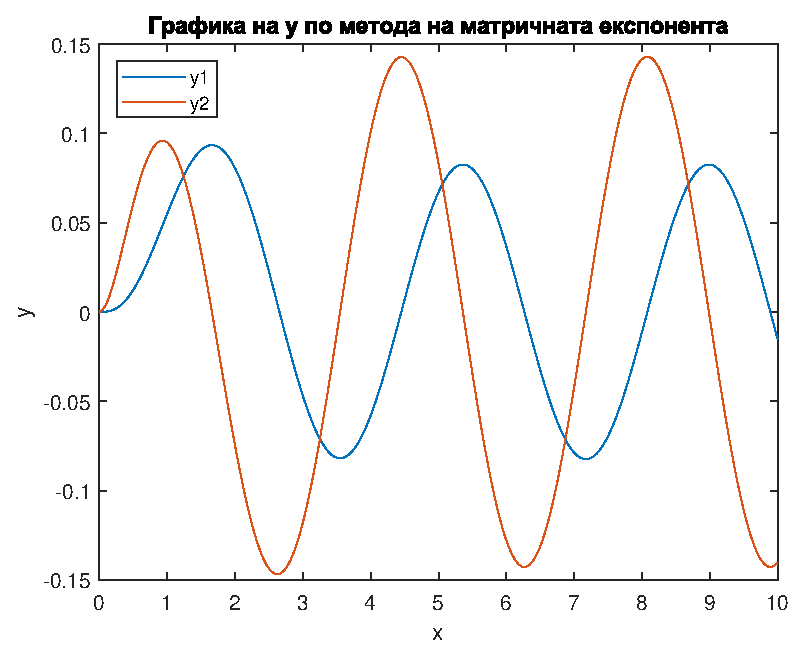
\includegraphics[width=4in]{secondTask_01.eps}
\end{center}

\newpage
\subsection{Задача 3}
Метода на крайните разлики се използва за решаване на обикновенни диференциални уравнения от вида 
\begin{equation*}
	x''(t)=f(t,x,x') \qquad t \in [a;b] \qquad x(a) = \alpha \qquad x(b) = \beta
\end{equation*}
Метода се състои в следните стъпки
\begin{enumerate}
\item Заменят се производните с техните приближения чрез крайни разлики
	\begin{equation*}
	x'(t) = \frac{y_{i+1} - y_{i-1}}{2h} \qquad \qquad x''(t) = \frac{y_{i+1} - 2y_i + y_{i-1}}{h^2} \qquad \qquad x(t_i) = y_i
	\end{equation*}
\item Решаване на системата от уравнения.
	\begin{equation*}
		\begin{array}{|l@{}}
			y_0 = \alpha\\ 
			\frac{y_{i+1} - 2y_i + y_{i-1}}{h^2} =  f \left(t_i, y_i, \frac{y_{i+1} - y_{i-1}}{2h}\right),  1\leq i \leq n-1 \\
			y_n = \beta
		\end{array}
	\end{equation*}
\end{enumerate}
но тази система е доста трудоемка за решаване. Задачата има вида
	\begin{equation*}
	a(t)x'' + b(t)x'+c(t)x=d(t) \qquad a(t) = 1 \quad  b(x) = \frac{1}{t} \quad  c(t) = \left( \frac{16}{t^2}\right) 
\quad d(t) = \sin \left( \frac{1}{t^2}\right)
	\end{equation*}
Можем да заместим производните с техните приближения. Ще положим 
	\begin{gather*}
	a_i = a(t_i) \qquad b_i = b(t_i) \qquad c_i = c(t_i) \qquad d_i = d(t_i) \\
	a_i \frac{y_{i+1} - 2y_i + y_{i-1}}{h^2} + b_i \frac{y_{i+1} - y_{i-1}}{2h} + c_i y_i = d_i \\
	y_{i-1} \left(\frac{a_i}{h^2} - \frac{b_i}{2h} \right) + 
	y_i \left( - \frac{2a_i}{h^2} + c_i \right) + 
	y_{i+1}\left(\frac{a_i}{h^2} + \frac{b_i}{2h} \right) = d_i \qquad \qquad \Big| \cdot -h^2 \\
	y_{i-1} \left(-a_i + \frac{hb_i}{2} \right) + 
	y_i \left(2a_i - c_i h^2 \right) + 
	y_{i+1} \left(-a_i - \frac{hb_i}{2} \right) = -h^2 d_i \\
	A_{i,i-1} = -a_i + \frac{hb_i}{2} = \frac{h}{2t_i} - 1 \qquad 
	A_{i,i} = 2a_i - c_i h^2  = 2-\frac{16h^2}{t_i ^2} \\
	A_{i,i+1} = -a_i - \frac{hb_i}{2} = - \frac{h}{2t_i} - 1 \qquad 
	f_i = -h^2 d_i = -h^2 \sin \left( \frac{1}{t^2}\right)
	\end{gather*}
\newpage

\begin{verbatim}
function thirdTask
a = 1; b = 4; % граници на интервала
alpha = -0.3; beta = 0.4; %x(a)=alpha; x(b)=beta
n = 100; % итерации
h = (b-a)/(n+1); % стъпка
t=a:h:b;
% Дефиниране на матрицата на коефициентите и вектора на дясната страна
A = zeros(n,n); f = zeros(n,1);
for i = 1:n
    if i ~= 1; A(i,i-1) = h/(2*t(i)) - 1; end
    A(i,i) = 2 - (16*h^2)/(t(i)^2);
    if i ~= n; A(i,i+1) = -h/(2*t(i)) - 1; end
    f(i) = -h^2*sin(1/t(i)^2);
end
% Прилагане на граничните условия
A(1,:) = 0; A(1,1) = 1;
A(n,:) = 0; A(n,n) = 1;
f(1) = f(1) - alpha*(h/(2*t(1)) - 1);
f(n) = f(n) - beta*(-h/(2*t(n)) - 1);
% Решаване на системата
x = A\f;
figure(3),plot(t,[alpha;x;beta]);
xlabel('t'); ylabel('x(t)'); title('Решение по метода на крайните приближения');
end
\end{verbatim}
\begin{center}
  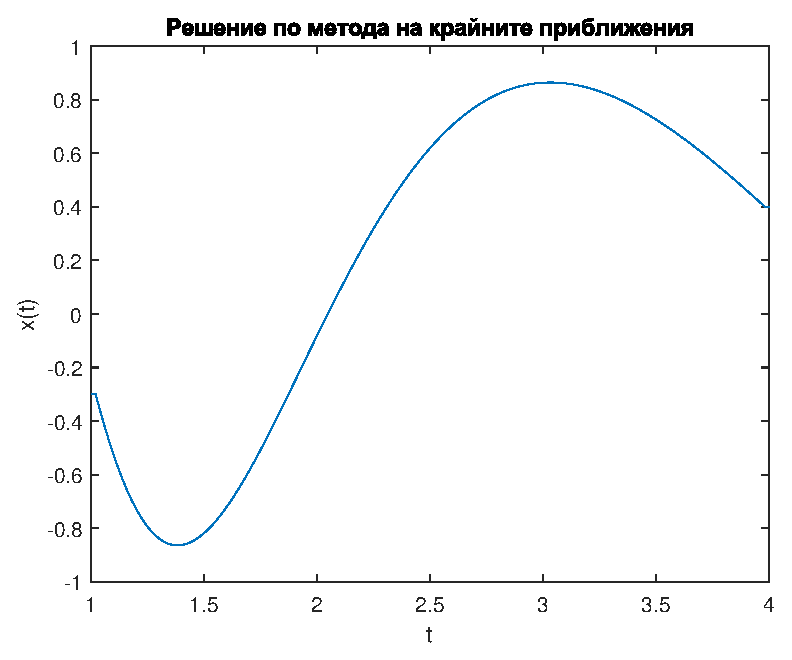
\includegraphics[width=4in]{thirdTask_01.eps}
\end{center}

\newpage
\subsection{Задача 4}
Метода на стрелбата се използва за решаване на обикновенни диференциални уравнения от вида
\begin{equation*}
	x''(t)=f(t,x,x') \qquad t \in [a;b] \qquad x(a) = \alpha \qquad x(b) = \beta
\end{equation*}
Метода се състои в следните стъпки
\begin{enumerate}
\item Представяне на началната задача като система от две уравнения от първи ред
	\begin{equation*}
		\begin{array}{|l@{}}
		 x'=y\\
		 y'= f(t,x,x')
		\end{array}\qquad \qquad  \text{при} \qquad \qquad 
		\begin{array}{|l@{}}
		x(a)=\alpha\\
		x(b)=\beta \\
		y(1) = y(4) = s
		\end{array}
	\end{equation*}
\item Задаваме си начално предположение за стойността на параметъра $s=a$.
\item \label{3}Решаваме получената система от диференциални уравнения с началните условия, използвайки числен метод.
\item Изчисляваме стойността на функцията получената от \ref{3}. функция $x$ в $t=b$.
\item Изчисляваме разликата между изчислената стойност на $x$ в края на интервала и действителната стойност на $x$ в краен момент, която е дадена в началните условия.
\item \label{6} Коригираме началното предположение за параметъра.
\item Повтаряме стъпки стъпки \ref{3} - \ref{6}, докато корекцията не стане достатъчно малка.
\end{enumerate}
\newpage

\begin{verbatim}
function fourthTask
t0=0;
t0=fsolve(@function1,t0);
x0=[-0.3,t0];
[t,x]=ode45(@function2,[1,4],x0);
figure(4),plot(t,x(:,1),t,x(:,2),'r')
xlabel('t');
ylabel('x(t)');
legend('x(t)',"x'(t)", 'Location', 'best');
title('Решение по метода на стрелбата');
end

function f=function1(x)
x0=[-0.3,x];
[t,x]=ode45(@function2,[1,4],x0);
n=length(t);
f=x(n,1)-0.4;
end

function dx=function2(t,x)
dx(1,1)=x(2);
dx(2,1)=sin(1/t^2)-(16/t^2)*x(1)-(x(2)/t);
end
\end{verbatim} 

\begin{center}
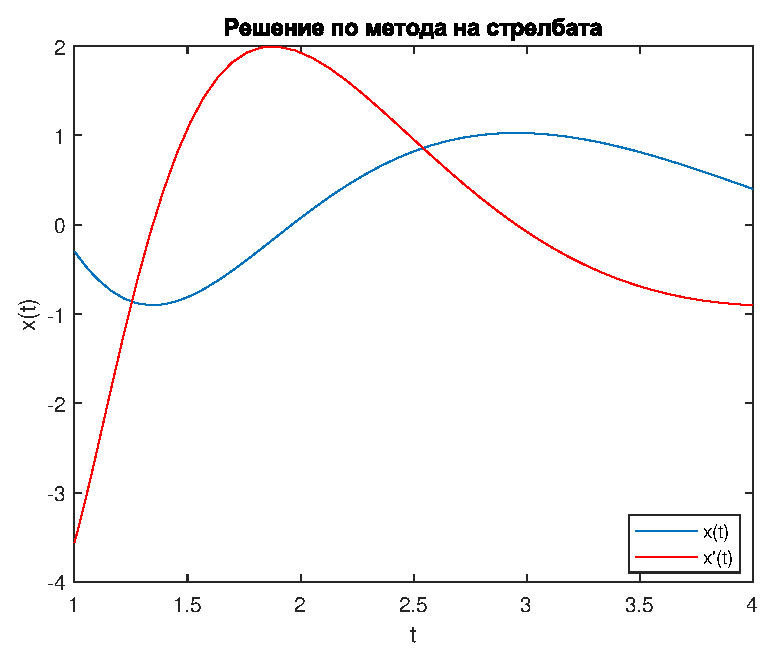
\includegraphics [width=4in]{fourthTask_01.eps}
\end{center}









































































\end{document}